\ofsubsection{Raças}
%
\ofquote{"Acredito que nos ache meio... estranhos, não é? Tudo bem. Nós, os Guado, estamos acostumados a isso.
Se quiser saber, vocês humanos nos são completamente nojentos. Ainda assim, que isso importa? Esse tipo de besteira está abaixo de nós, não? Uma vez, uma criança humana apenas olhou para mim e então começou a chorar. Isso me magoou."}{Guado fêmea}\\
%
\vfill
%
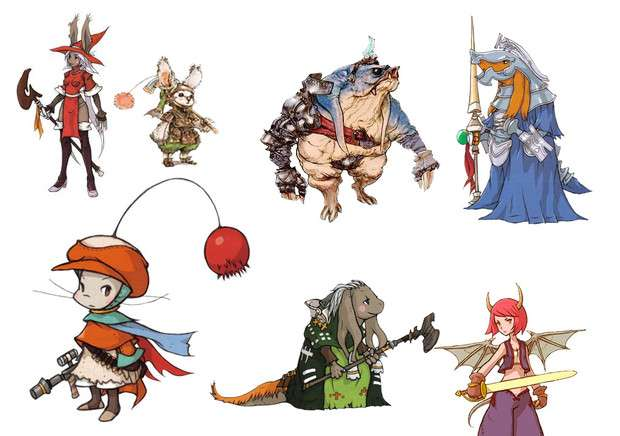
\includegraphics[width=\columnwidth]{./art/races/races.jpg}
%
\vfill
%
Geralmente, nos diferenciamos entre dois tipos de criaturas vivas: personagens, que por padrão, assumimos serem humanos e os monstros, estes que supomos serem similares aos animais.
Assim como no mundo real, alguém pode identificar diferentes tribos e raças dentro daqueles grupos e quanto aos monstros, apresentamos uma ampla variedade de espécies diferentes no bestiário.
A seguir, exploraremos as raças de personagem ficcionais, mas que lembram humanos tanto na aparência quanto na inteligência.
Estas, intituladas \accf{Raças humanoides} podem ser interessantes para ambos os jogadores e mestres de jogo, porque eles aumentam a diversidade do mundo, enquanto ainda cumprem os mesmos papéis que os humanos.
%
\vfill
%
\ofquote{"Nós anões temos um ditado: Seja forte. Mas se as coisas parecerem perigosas, fuja e seja forte outro dia. \\}{Anão}\\\\
%
Como MJ, você pode criar várias raças humanoides para compor a população de seu mundo.
Normalmente, aquelas raças se encaixam em algo entre humanos e monstros.
Por um lado, eles são inteligentes, podem interagir e se comunicar com humanos e criar suas próprias civilizações e tecnologias.
Por outro lado, elas podem variar enormemente em aparência, língua, aspectos e jeito de viver comparado aos humanos.
Além do mais, as raças com anatomias diferentes podem preferir condições de vida que são desagradáveis aos humanos, como submersos, subterrâneos ou no topo de árvores.
Naturalmente, a existência de tais raças diferentes terão consequências no estado do mundo: assim como tribos humanas, outras raças podem criar conflitos e alianças entre si mesmos e um com o outro.
Portanto, cada raça escreverá seu história única e moldar o mundo à sua próprio interesse.
%
\newpage
%
\ofquote{"Tenho que descobrir quem sou. Estou assustado, e se eu não for humano?"}{Vivi}\ofpar
%
Como habitantes do mundo de jogo, os personagens dos jogadores também podem ser parte de uma raça humanoide que exista nele.
Portanto, é importante que o MJ introduza brevemente as raças existentes aos jogadores antes deles criarem seus personagens.
Quando um jogador decidir que seu personagem é de uma raça não humana, isso implica em algumas consequências:
primeiro, é importante que o jogador considere a raça de seu personagem e origem como parte de sua história.
Portanto, a aparência de um personagem será altamente influenciada pela sua raça e eles podem mostrar traços de personalidade específicos comuns àqueles de seu povo.
Durante a aventura, os membros do grupo de raças diferentes podem ser percebidos e tratados de formas distintas, a depender de com quem interagem.
%
\vfill
%
A escolha da raça não deve mudar fundamentalmente as mecânicas do jogo para os personagens jogadores.
No entanto, é benéfico explorar elementos de jogabilidade que ajudam aos jogadores a considerar suas raças de personagem enquanto interpretam.
Cada raça comumente tem pelo menos um ofício ou disciplina na qual se destacam, normalmente permitido pela sua anatomia ou conhecimento único.
Tal perícia pode ser expressada através de Talentos exclusivos da raça, os chamados \accf{Talentos raciais}.
Eles funcionam exatamente como os Talentos comuns, mas estão disponíveis apenas para os personagens de raças específicas.
Quando os jogadores criarem seus personagens, eles podem escolher um deles;
A seguir, alguns exemplos de raças humanoides são mostradas, as quais são inspiradas naquelas que aparecem em vários jogos de Final Fantasy.
Eles devem servem como exemplos e ao MJ não é esperado inclui-los como parte do mundo que criem.
O propósito principal é de fornecer inspiração para que se criem as suas próprias.
Por fim, note que dois Talentos raciais são dados para cada exemplo a fim de que os jogadores escolham entre eles.
%
\vfill
%
\ofboxwithtitle{Exemplo: Talentos raciais} 
{
	Kimahri Ronso é um guardião da Invocadora Yuna, a quem jurou proteger em sua peregrinação.
	Quando um jovem chamdo Tidus também tentou se tornar seu guardião, ele decidiu testar seu poder de combate.
	Escondeu-se no topo de algumas ruínas a sua espera a fim de emboscá-lo.
	O MJ pede que ambos façam um teste para decidir se a emboscada foi ou não bem sucedida.
	Kimahri tem o Talento racial Caçador poderoso para os Ronso, então tem vantagem nesse teste.
	Ele rola [1,~5,~4] enquanto Tidus [3,~2].
	Portanto, o MJ decide que Tidus foi pego de surpresa  Kimahri começa a batalha com uma rodada surpresa.
}
%
\clearpage
%
%
\ofquote{"É preciso coragem para chamar um Bangaa de lagarto!"\\}{Bangaa macho}
%
\begin{center} 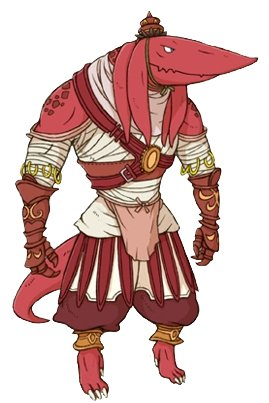
\includegraphics[width=0.88\columnwidth]{./art/races/bangaa.jpg} \end{center}
%
Com sua pele coberta em escamas, assim como suas longas cabeça e cauda, o \accf{Bangaa} claramente lembra um lagarto.
Outra característica notável deles são suas quatro longas orelhas que recaem sobre a lateral de seu rosto.
O físico impressionante deles e traços incomuns os fazem parecer intimidante perante outras raças.
Mesmo assim, eles são bem inteligentes. A anatomia de suas bocas torna difícil para eles falar na linguagem humana apropriadamente.
Os Bangaa não têm estruturas sociais rígidas.
Geralmente, eles viajam ou residem em grandes cidades e não têm problemas em viver entre outras raças.
Embora sejam tradicionalmente guerreiros, muitos vão além disto em direção ao comércio, política ou artesanato.
Muitos Bangaas evitam a magia, mas podem compensar isso com sua força física e inteligência.
Também têm uma preferência a usar armas e armaduras bem feitas.
%
\\\\
%
\accf{Talento racial - Regenerar:} As escamas do Bangaa 
não somente o protegem de danos recebidos, mas também o ajudam e se recuperar de ferimentos muito mais rápido.
Após cada batalha vencida, imediatamente recupere uma quantidade de PV igual ao seu nível atual se não tiver sofrido KO.
%
\\\\
%
\accf{Talento racial - Força bruta:} Como uma das raças fisicamente mais formidáveis, você recebe vantagem em testes relacionados a empurrar, mover e quaisquer testes opostos de força.
%
%
\newpage
%
%
\ofquote{"Embora nós Guado sejamos diferentes em aparência aos humanos, nosso respeito pelos mortos é o mesmo."\\}{Guado macho}
%
\begin{center} 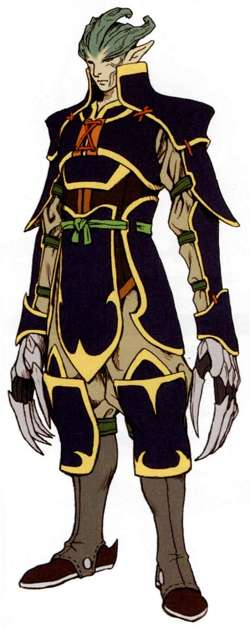
\includegraphics[width=0.5\columnwidth]{./art/races/guado.jpg} \end{center}
%
A maioria das características proeminentes dos \accf{Guado} são seus braços longos que terminam em dedos em forma de garras e suas orelhas longas.
O cabelo deles cresce de forma incomum e normalmente se compara a galhos de uma árvore.
Os Guado são levemente mais esbeltos e mais flexíveis do que os humanos, que os permitem ser incrivelmente ágeis.
No entanto, eles preferem vestir roupas longas ou armadura pesada. Normalmente estabelecem seus assentamentos em ambientes naturais como florestas e cavernas.
São uma raça religiosa que pratica rituais elaborados para celebrar os mortos.
O intitulado Maester é o religioso oficial e, de fato, o líder político da tribo.
Os Guado são extremamente bem versados em magia e preferem a usar ao invés da tecnologia.
Eles acreditam em si mesmo como sendo superiores às outras raças e em retorno são tidos como arrogantes.
%
\\\\
%
\accf{Talento racial - Além-mundo:} Os Guados têm uma conexão única com o mundo dos mortos, o qual eles chamam de Além-mundo. Você pode realizar um longo ritual de 10 minutos e se for bem sucedido no teste, você pode falar com o fantasma de um personagem morto.
A DF é determinada pelo MJ, mas fica mais fácil quanto mais próximo que você estiver do local de morte da pessoa, além do quanto mais íntimo a ela você tenha sido.
%
\\\\
%
\accf{Talento racial - Célere:} Os Guado recebem vantagem em corridas e testes opostos relacionados a velocidade.
%
\clearpage
%
\ofquote{"Um animal empalhado!? Vou te mostrar que eu sou um moogle, kupo!"}{Montblanc}
%
\begin{center} 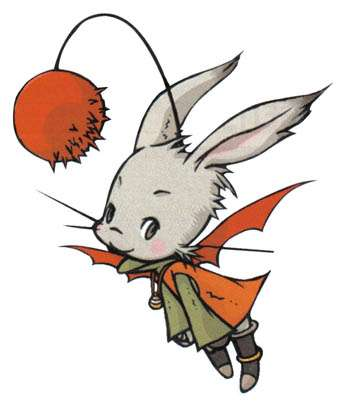
\includegraphics[width=0.8\columnwidth]{./art/races/moogle.jpg}  \end{center}
%
Os \accf{Moogle} são pequenos, geralmente não mais do que 1u e têm vozes bem agudas.
Com suas longas orelhas e sua pelugem, que podem ser quase de qualquer cor, eles lembram coelhos.
Além disso, eles têm pequenas asas em suas costas assim como uma antena na cabeça, com uma bola peluda na extremidade dela.
Esse "pom pom" é muito sensível ao toque e, portanto, os Moogle são normalmente muito protetivos quanto a eles.
Eles variam muito: enquanto alguns vivem em tribos escondidas em florestas, outros preferem viajar sozinhos ou viver em grandes cidades.
Também são uma raça ambiciosa que ama explorar e descobrir disciplinas diferentes.
Enquanto têm tradicionalmente dependência à magia para sobreviver, Moogles modernos também se tornam artífices, artistas, comerciantes e até mesmo guerreiros.
A dieta deles consiste em sua maioria de nozes e plantas, pois eles raramente comem qualquer tipo de carne.
Moogles são geralmente percebidos como gentis e confiáveis, mas com frequência não são levados a sério devido à sua aparência. 
%
\\\\
%
\accf{Talento racial - Planar:} Usar suas asas, Moogles podem voar até 0.5u acima do chão e podem cobrir uma distância de até 10u antes de aterrizar.
Enquanto voando, eles podem se mover apenas metade se comparado ao seu movimento normal.
Além do mais, eles podem planar de alturas até 10u de altura sem receber danos.
%
\\\\
%
\accf{Talento racial - Redemog:} Devido às suas habilidades mágicas, você é capaz de se comunicar telepaticamente com qualquer Moogle conhecido ou não Moogles dispostos com quem você compartilhe um vínculo, por exemplo com alguém de seu grupo.
%
\newpage
%
\ofquote{"É difícil quanto todos pensam em você como um gênio"\\}{Ezel}\\
%
\begin{center} 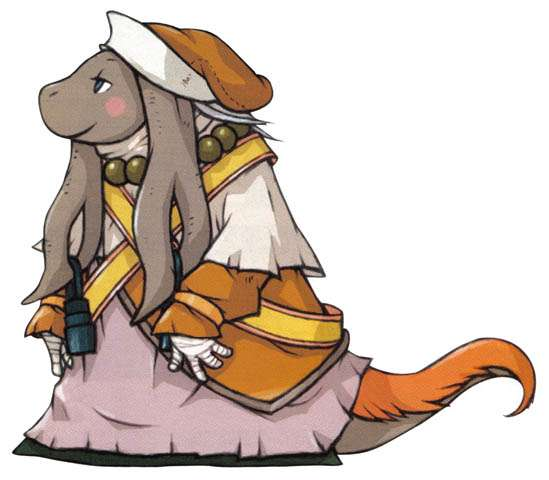
\includegraphics[width=\columnwidth]{./art/races/numou.jpg} \end{center}
%
Os \accf{Nu Mou} são levemente mais curtos do que as outras raças e a cor de suas peles suaves podem variar bastante.
Eles têm corpos bem redondos e rostos que, juntamente a suas caudas longas, lembram de animais caninos.
Suas longas orelhas se bifurcam perto da extremidade, deixando grandes buracos que normalmente decoram com brincos.
A média de expectativa de vida de um Nu Mou é significantemente mais longa do que qualquer outra raça, com alguns tendo vivido até mais de 300 anos.
Acredita-se que os Nu Mou são de longe a raça mais antiga existente, que já governaram sobre as civilizações mais ricas e poderosas.
Atualmente, os membros dessa raça estão espalhados ao redor do mundo com pouca coesão. 
Eles sempre têm sido usuários de magias altamente habilidosos, mas cada vez mais Nu Mous também têm mostrado interesse em pesquisar alquimia, astronomia e dominação de monstros.
A maioria deles tendem a ser introvertidos e focados em uma área de especialização, que é o porquê das outras raças os terem como seres estranhos, mas inofensivos.  
%
\\\\
%
\accf{Talento racial - Sabedoria antiga:} resquícios da sabedoria Nu Mou sobreviveu através dos séculos e ainda são conhecidas entre os seus membros.
Portanto, você é capaz de ler e entender quase que qualquer linguagem ou dialeto antigo indiferente de quanto tempo não sejam usadas.
%
\\\\
%
\accf{Talento racial - Nobre Nu Mou:} como um membro de um clã Nu Mou, você é mais inteligente quanto às artes mágicas. Você sempre pode identificar qualquer magia ou efeito máfico similar a alguns dos seus e receber Vantagem quanto tentar identificar magias não familiares. 
%
\clearpage
%
\ofquote{"Você enfureceu Kimahri! Os espíritos do Ronso guiarão a lança de Kimahri!"}{Kimahri}
%
\begin{center} 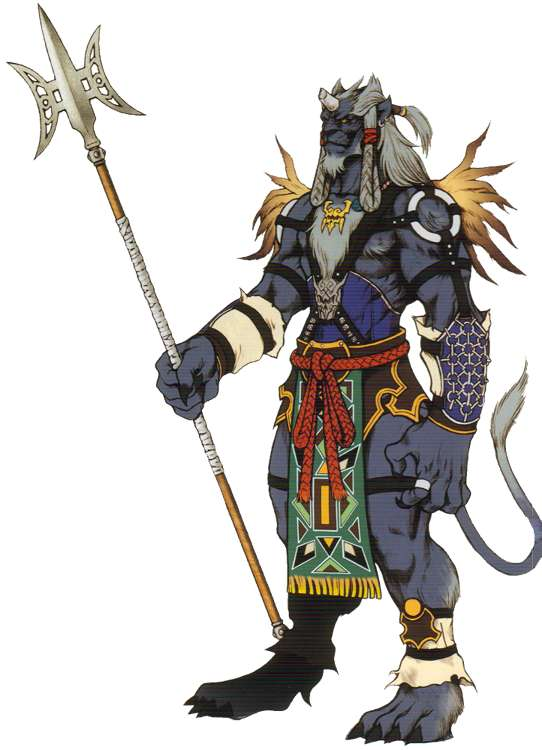
\includegraphics[width=\columnwidth]{./art/races/ronso.jpg} \end{center}
%
Os \accf{Ronso} parecem como uma mistura entre humanos e leões.
Enquanto apresentam muitas características felinas como garras e uma cauda, seus maneirismos são mais próximos aos humanos.
Contudo, se diferenciem pelos seus pelos azulados e seus chifres na testa.
Eles preferem roupas leves, pois seu pelo já cobrem todo o seu corpo.
As tribos Ronso preferem viver em climas frios, normalmente no topo de montanhas, que consideram ser sagradas.
Eles são uma raça de guerreiros primariamente e que raramente lidam com magia ou tecnologia. Tendem a ser religiosos e têm um orgulho especial de seus chifres, o qual entendem como a fonte de sua força.
Apesar disso, eles normalmente são indiferentes à forasteiros e ocasionalmente se metem com outras raças e civilizações em termos amigáveis.
Portanto, os Ronso são tidos como um povo gentil, mas primitiva.
%
\\\\
%
\accf{Talento racial - Pele dura:} A pelugem espessa permite aos Ronso estar confortável independente do ambiente ao seu redor.
Você não fica lento devido a terreno difícil como pântanos ou neve e você não necessita de abrigo mesmo sobre condições climáticas extremas.
%
\\\\
%
\accf{Talento racial - Poderoso caçador:} como uma espécie carnívora, os Ronso se tornaram caçadores por excelência. Tenha vantagem em rolagens que envolvam tanto perseguir quanto evitar ser notado pela sue presa.
%
\newpage
%
\ofquote{"As Viera podem começar como parte da floresta, mas não é o único fim que podemos escolher."}{Fran}
%
\begin{center} 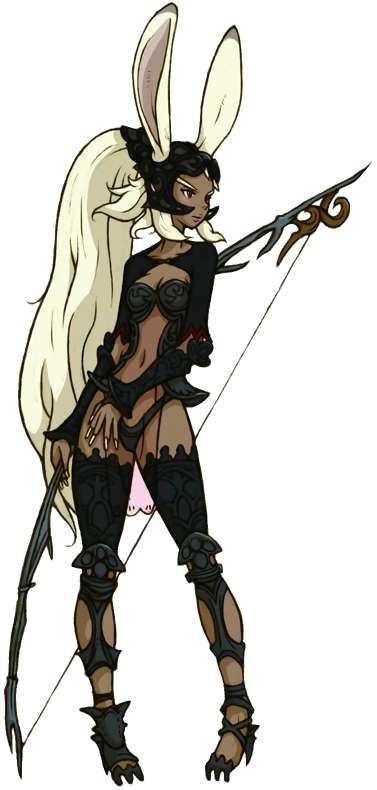
\includegraphics[width=0.58\columnwidth]{./art/races/viera.jpg} \end{center}
%
As \accf{Viera} se parecem com os humanos, exceto por algumas de suas características: orelhas longas e cobertas por pelos, mãos com garras e pés pontudos, reminiscencias de membros felinos.
A maioria das Viera vestem luvas e salto altos que são feitos para se ajustar à sua anatomia única.
Em geral, preferem roupas leves e reveladoras que não impedem seu movimento.
Suas tribos vivem em florestas que são fechadas ao resto do mundo.
Não somente consideram esse bioma como seu próprio, mas também sentem uma conexão espiritual à sua flora e fauna. 
Assim, normalmente não se relacionam com outras raças e são hostis a forasteiros.
Aquelas que decidem deixar a floresta são imediatamente consideradas exiladas e tratadas como forasteiros.
Enquanto suas tribos consistam em sua maioria de caçadores e coletores, alguns também têm uma forte afinidade à magia.
Vieras exiladas são com frequência não tão proficientes em suas disciplinas tradicionais, mas podem possuir uma variedade de habilidades devido a suas experiencias em outras civilizações.
%
\\\\
%
\accf{Talento racial - Naturalmente perceptiva:} as Viera tem os sentidos muito mais aguçados do que as outras raças. 
Tenha vantagem em todos os testes que envolvam perceber sons, cheiros, rastros e movimentos ao seu redor.
%
\\\\
%
\accf{Talento racial - Proscrito da floresta:} como um dos Viera que abandonaram seu lar ancestral, você aprendeu a sobreviver ao aprimorar sua arte. Você é adepta a identificar ervas, montar acampamento e disfarçar suas localizações anteriores, tendo vantagem em tais testes.
%
\clearpage
%
\ofquote{"Quando uma pessoa tem alguém com quem se preocupa tanto, sacrificar-se é algumas vezes o mínimo que se pode fazer e, talvez, isso é o que nos faz humanos."}{Vincent}
%
\begin{center} 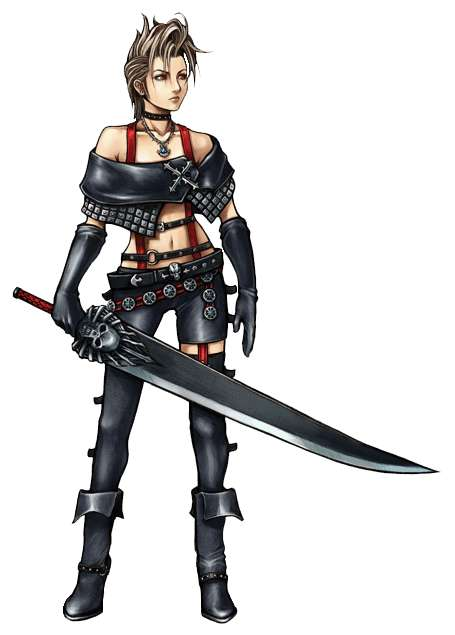
\includegraphics[width=0.9\columnwidth]{./art/races/human.jpg} \end{center}
%
Os \accf{Humanos}, além de qualquer coisa, são tão adaptáveis e aventureiros como suas contra partes do mundo real.
Vindo de aparentemente todo mundo no multi-verso, estes seres têm a tendência a serem ambiciosos, astutos, inquisitivos e têm gerado tantos heróis quanto vilões!
De fato, sua ambição pelo auto aprimoramento e de apenas saber parece ilimitada. 
Como um testamento de sua ambição pelo poder, a humanidade é uma das espécies mais prevalentes a serem encontradas em muitos planetas e planos.
Uma das forças da humanidade é a impressionante variedade de línguas e instituições sociais que possuem.
Diz-se que isso explica sua convicção em liberdade individual, embora também resulte em uma relativa falta de solidariedade e coesão de grupo.
\\\\
\accf{Talento racial - Força de vontade:} algumas pessoas são guiadas pelo desejo pela perfeição e auto aprimoramento, deixando nada em seu caminho, salvo sua bússola moral. Você é uma dessas pessoas, com o sangue de conquistadores correndo através de suas veias. Tenha vantagem em testes relacionados a negociação e liderança.
\\\\
\accf{Talento racial - Por um fio:} seja uma benção, destino ou mera reflexão de sua essência interior, muitos humanos têm uma aptidão incomum a sobreviver aos maiores dos perigos e você não é uma exceção. Sempre que passar um teste no qual teve desvantagem, tenha vantagem em qualquer outro próximo que realize.
%
\pagebreak\\
%
\ofquote{"uuuaaah...Quer lutar? Depois desse mapa, talvez..."\\}{Miqo'te macho}
%
\begin{center} 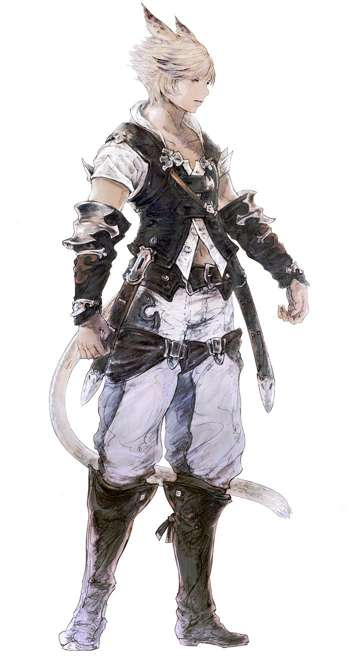
\includegraphics[width=0.7\columnwidth]{./art/races/miqote.jpg} \end{center}
%
Uma espécie de humanoides felinos, os \accf{Miqo'te} são muito poucos em número e mais insulares do que as outras raças.
Com suas orelhas pronunciadas e caudas cobertas de pelo, eles aparentam uma mistura entre humanos e gatos.
Contudo, diferente de outras raças, preferem se vestir muito parecido com os humanos.
A maioria deles vivem em tribos isoladas com estruturas hierárquicas rígidas, mas alguns também se integraram com sucesso em outras culturas.
Tradicionalmente, o Miqo'te venera o sol e a lua como seus deuses.
Uma ampla variedade de personalidades é representada dentro desta raça: alguns são astuciosos, impetuosos e facilmente entediados enquanto outros são mais reservados e taciturnos, embora tanazes. 
Os Miqo'te são bem adaptados a vários ambientes, seja selva, deserto ou planícies e possuem habilidades impressionantes em caça e pesca devido à sua enorme destreza.
\\\\
\accf{Talento racial - Reflexos gatunos:} sua maior benção são seus olhos, orelhas e sua cauda.
Tenha vantagem em testes que envolvam espreitar sua presa e equilíbrio, enquanto ignora desvantagem devido à escuridão.
\\\\
\accf{Talento racial - Nove vidas:} algumas vezes você apenas não consegue se manter morto.
Sempre que sofrer KO, recupere-se disso ao descansar por 1 hora ao invés de precisar de uma noite completa de sono.
%
%
\clearpage
